\documentclass[a4paper]{article}
  %!TEX root = POR_Caso2.tex
%% Jose Javier Gonzalez Ortiz %%
%% Core default Configuration %%
%% 2016-07-07                 %%

%%%%%%%%%%%%
% PACKAGES %
%%%%%%%%%%%%

\usepackage[T1]{fontenc} % Use 8-bit encoding that has 256 glyphs
\usepackage[utf8]{inputenc} % For Spanish characters
\usepackage[english,spanish,es-noshorthands,es-tabla]{babel}  % English localisation
% \usepackage[spanish, es-noshorthands,es-tabla]{babel}               % Spanish hyphenation and document rules


% =========== General Formatting =============
\usepackage[left=2.5cm, right=2.5cm, top=2.5cm, bottom=2cm]{geometry} % Margin sizes
\usepackage{microtype} % Slightly tweak font spacing for aesthetics
% \usepackage{fancyhdr} % Allows for nice header and footer
% \usepackage{sectsty} % Allows customizing section commands
% \usepackage{titlesec} % Allows customization of section titles
% \usepackage{appendix} % Enables appendices
% \usepackage{enumerate} % Custom numerate, useful for i,ii,iii... I,II,III...
% \usepackage{relsize} % Defines several commands to set font sizes relative to the current size. Useful for enlarging math
\usepackage{setspace} % Sup­port for set­ting the spac­ing be­tween lines in a doc­u­ment. \sin­glespac­ing, \one­half­s­pac­ing, and \dou­blespac­ing
% \usepackage{changepage} % To change relative geometry of particular pages
% \usepackage[usenames,dvipsnames]{xcolor} % Required for custom colors

% =========== Linking =============
\usepackage{hyperref} % For hyperlinks in the PDF
\hypersetup{
    colorlinks = false,
    linkcolor = red,
    urlcolor  = blue,
    citecolor = green,
    filecolor = cyan,
    anchorcolor = black
}
% =============== Math ===============
\usepackage{amsmath} % Standard math packages
\usepackage{amsthm} % Math Theorems
\usepackage{amssymb} % Math Symbols
\usepackage{amsfonts} % Math Fonts
% \usepackage{upgreek} % Nice sigma => \upsigma
\usepackage{array} % Enables array features
% \usepackage{siunitx} % For SI Unit easy formatting

% =============== Figures ===============
\usepackage{graphicx} % Image insertion.
\usepackage{float} % % Required for tables and figures in the multi-column environment - they need to be placed in specific locations with the [H] (e.g. \begin{table}[H])
% \usepackage{wrapfig} % Al­lows fig­ures or ta­bles to have text wrapped around them
% \usepackage{rotating} % Allows for sideways figure with twoside recognition

% =============== Tables ===============
\usepackage{booktabs} % Horizontal rules in tables
% \usepackage{multirow} % Combined rows in tables
% \usepackage{multicol} % Combined columns in tables
\usepackage{colortbl} % Color cells
\usepackage{longtable} % Tables than span multipages

% ============ Bibliography ============
\usepackage{csquotes}% Recommended package for biblatex
% Use biblatex as the bibliography package.
% The specific settings emulate the tradional bibtex alpha style
% \usepackage[backend=bibtex]{biblatex}


% ============ Glossaries ============
% \usepackage[acronym]{glossaries} % Very good package to create glossaries, acronym lists or symbols (nomenclature) lists.

% =============== Footnotes ===============
\usepackage{footnote}
\makesavenoteenv{figure} % Footnotes in Figures are displayed correctly
\makesavenoteenv{table} % Footnotes in Tables are displayed correctly

% =============== Other ===============
% \usepackage{datetime} % Date-Time formatting
% \usepackage{ulem} % For strikethrough text \st{}
% \normalem %Restores the emphasis to italics after ulem
\usepackage{textcomp} %Text Com­pan­ion fonts

\usepackage{pdfpages} % Insert pdfs
% \usepackage{lipsum} % Used for inserting dummy 'Lorem ipsum' text into the template
% \usepackage{lettrine} % The lettrine is the first enlarged letter at the beginning of the text
\usepackage{pdflscape} % Individual horizontal pages
%\usepackage[space]{grffile} % insert files with spaces
%\usepackage{xargs} % Expanded arguments features
%\usepackage{fix-cm} % Computer-Modern at arbitrarysizes
\usepackage{eurosym} % Eurosymbol
%\usepackage{watermark} % To use display water marks in the document

%%%%%%%%%%%%
% CAPTIONS %
%%%%%%%%%%%%
\usepackage[hang, small,labelfont=bf,up]{caption} % Custom captions under/above floats in tables or figures
\usepackage{subcaption} % For custom caption environments
    % \numberwithin{equation}{section} % Number equations within sections (i.e. 1.1, 1.2, 2.1, 2.2 instead of 1, 2, 3, 4)
    % \numberwithin{figure}{section} % Number figures within sections (i.e. 1.1, 1.2, 2.1, 2.2 instead of 1, 2, 3, 4)
    % \numberwithin{table}{section} % Number tables within sections (i.e. 1.1, 1.2, 2.1, 2.2 instead of 1, 2, 3, 4)


%%%%%%%%%%%%%%%%%
% MATH COMMANDS %
%%%%%%%%%%%%%%%%%
% Macros mathematical delimiters
\usepackage{mathtools} % Extra math tools such as PairedDelimiter
% To get automatically sized delimiters follow the command with an asterisk
% e.g  \norm*{\sin\paren*{\frac{1}{2}}}
    \DeclarePairedDelimiter\paren{(}{)} % Parenthesis Macro
    \DeclarePairedDelimiter\bra{[}{]} % Bracket Macro
    \DeclarePairedDelimiter\curly{\{}{\}} %Curly Brackets
    \DeclarePairedDelimiter\abs{\lvert}{\rvert} % Single vertical lines, absolute values
    \DeclarePairedDelimiter\norm{\lVert}{\rVert} % Double vertical values, norm
    \DeclarePairedDelimiter\floor{\lfloor}{\rfloor} % Floor deilimiters
    \DeclarePairedDelimiter\ceil{\lceil}{\rceil} % Ceiling delimiters

%Other useful macro symbols
    \newcommand{\grad}{\nabla} % For gradients
    \newcommand{\deriv}[2]{\frac{d #1}{d #2}} %Derivative macro
    \newcommand{\pderiv}[2]{\frac{\partial #1}{\partial #2}} % Partial derivative macro
    \newcommand{\bigO}{\mathcal{O}} % For fancy Big O notation
    \newcommand{\gm}[1] {\guillemotleft #1\guillemotright} %$ pretty gimollet <<sth>>

%%%% Vector symbols
% Really useful when doing vector calculus or machine learning
    % \newcommand{\vx}{\bar{x}}
    % \newcommand{\vv}{\bar{v}}
    % \newcommand{\vw}{\bar{w}}
    % \newcommand{\vu}{\bar{u}}
    % \newcommand{\vy}{\bar{y}}
    % \newcommand{\vt}{\bar{\theta}}

%%%%%%%%%%%%%%%%%%%%%
% REVISION COMMANDS %
%%%%%%%%%%%%%%%%%%%%%
% \usepackage[colorinlistoftodos]{todonotes} % useful for leaving todonotes

% % Todo Commands \hightodo, \lowtodo
%     \newcommand{\hightodo}[1]{\todo[inline,backgroundcolor=red!90!yellow!80!white]{\textbf{\userId}: #1}}
%     \newcommand{\lowtodo}[1]{\todo[inline,backgroundcolor=blue!30!white]{\textbf{\userId}: #1}}

% Tip box environments
% \usepackage{tcolorbox} % Color boxes for comment
% \newtcolorbox{tip}{colback=blue!5!white,colframe=blue!75!black} % Vanilla tip box
% \newtcolorbox{tipt}[1]{colback=blue!5!white,colframe=blue!75!black,fonttitle=\bfseries,title=#1} % Tip box with title

% % Thick strike out line
%     \newcommand{\soutthick}[1]{%
%         \renewcommand{\ULthickness}{3pt}%
%            \sout{#1}%
%         \renewcommand{\ULthickness}{.4pt}% Resetting to ulem default
%     }

%%%%%%%%%%%%
% QUOTE    %
%%%%%%%%%%%%

\makeatletter
\newenvironment{chapquote}[2][2em]
  {\setlength{\@tempdima}{#1}%
   \def\chapquote@author{#2}%
   \parshape 1 \@tempdima \dimexpr\textwidth-2\@tempdima\relax%
   \itshape}
  {\par\normalfont\hfill--\ \chapquote@author\hspace*{\@tempdima}\par\bigskip}
\makeatother



% Define blank page

\newcommand\blankpage{%
    \mbox{}%
    \thispagestyle{empty}%
    \newpage%
}

% Epigraph left side (good for quotes or dedications)

% \usepackage{epigraph}

% \setlength\epigraphwidth{8cm}
% \setlength\epigraphrule{0pt}
% \makeatletter
% \patchcmd{\epigraph}{\@epitext{#1}}{\itshape\@epitext{#1}}{}{}
% \makeatother


%%%%%%%%%%%%
% UNITS    %
%%%%%%%%%%%%

% \DeclareSIUnit{\EUR}{\text{\euro}}
% \sisetup{
  % per-mode = symbol,
  % inter-unit-product = \ensuremath{{}\cdot{}}, % Cdot between units
% }
  \usepackage{parskip}
  % \addbibresource{mybib.bib}
    %\usepackage{nameref}
    %\usepackage{tabularx}
  % \usepackage{array}
  \usepackage{fancyhdr}
  \lhead{Arquitectura de Sistemas en Red}
  \rhead{Desarrollo de una aplicación con Bluemix}

% Global variables
  \newcommand{\HWTitle}{Desarrollo de una aplicación con Bluemix}
  \newcommand{\HWDueDate}{\today}
  \newcommand{\HWAuthorName}{José Javier González Ortiz \and Lucía Montero Sanchis}
  \title{\HWTitle \\ \vspace{.25cm}}
  \date{\HWDueDate}
  \author{\HWAuthorName}

\usepackage{graphicx}
\usepackage{wrapfig}
\usepackage{lscape}
\usepackage{rotating}
\usepackage{epstopdf}

\begin{document}
\maketitle
\pagestyle{fancy}
\vfill
%\listoffigures
\vfill\vfill
\newpage
\section{Introducción} % (fold)
\label{sec:introducción}
  Se ha desarrollado una aplicación Flask basada en Python, con los siguientes cinco servicios:
  \begin{itemize}
    \item Language Translator
    \item Visual Recognition
    \item Text to Speech
    \item Natural Language Understanding
    \item Cloudant NoSQL DB
  \end{itemize}
  El objetivo de la aplicación es ofrecer un servicio de análisis de imágenes y de frases en diferentes idiomas.

  La aplicación usa cookies para mantener historial de usuarios de forma independiente. Se soporta también url estáticas para búsquedas ya realizadas. Esto permite poder compartir o salvar búsquedas previas.

  Se ha empleado AJAX para las pantallas de carga y para obtener el historial de los usuarios. La aplicación soporta cacheado de resultados de cara a evitar repetir peticiones en un espacio de tiempo corto debido al alto numero de comunicaciones de microservicios presentes. Esto agiliza mucho consultas del historial.

\begin{figure}[htp!]
    \centering
    \caption{La aplicación está disponible tanto en Bluemix como en una página web personal. El código está compartido en GitHub, y se ha utilizado TravisCI para la Integración Continua.}
    \label{fig:webs}
    
\includegraphics[width=\textwidth]{webs1}
\end{figure}
\section{Enlaces URL} % (fold)
\label{sec:enlaces_url}

% section enlaces_url (end)

\begin{figure}[htp!]
    \centering
    \caption{Bluemix: \url{http://erittely.josejg.com} \newline{} \url{http://erittely.eu-gb.mybluemix.net/} }
    \label{fig:blue}
    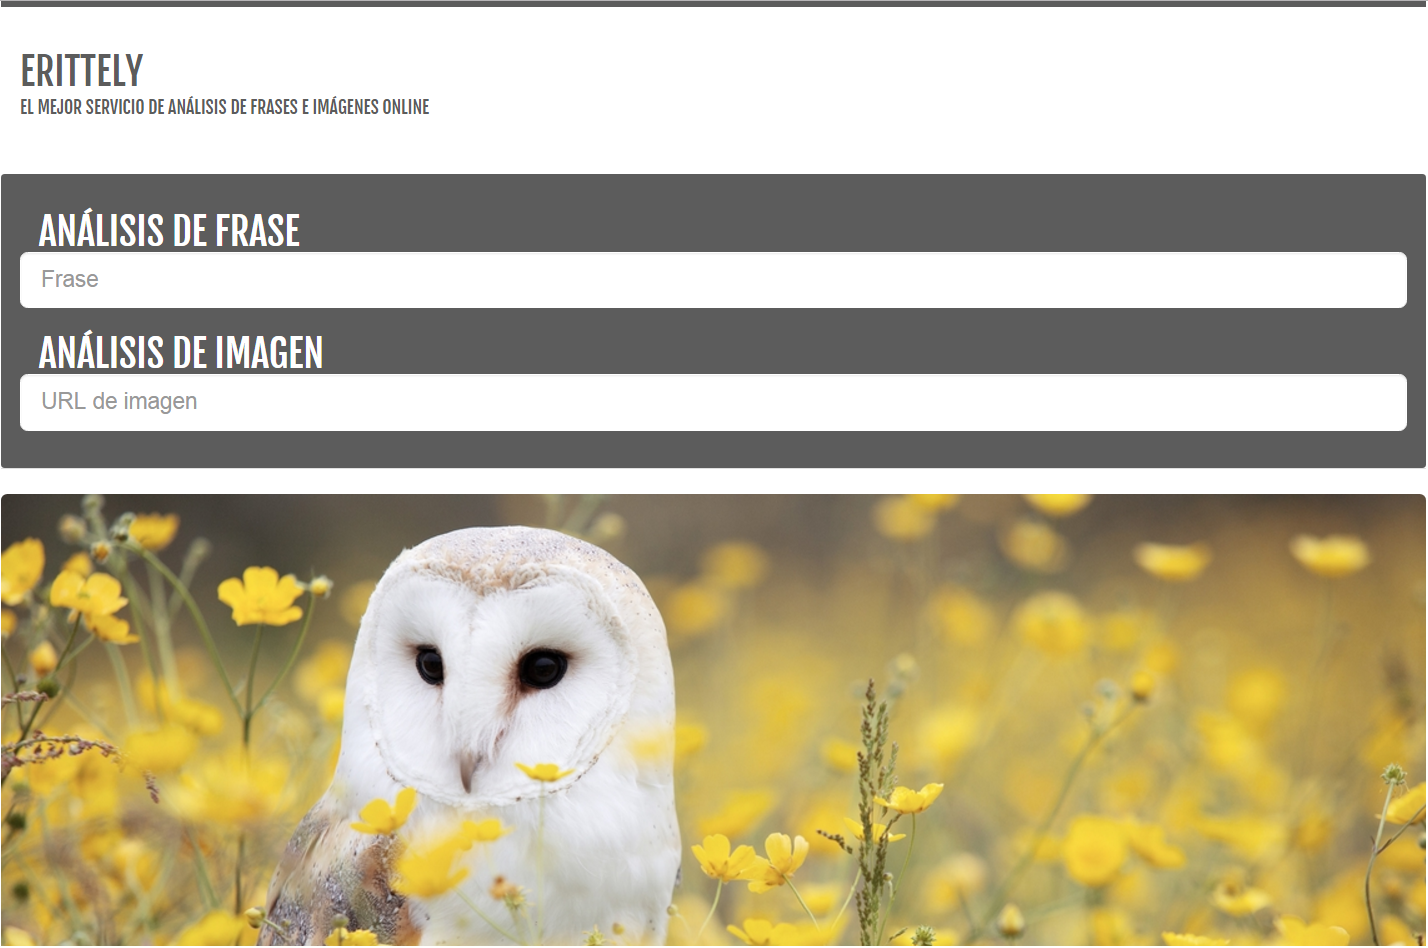
\includegraphics[width=\textwidth]{blue}
\end{figure}


\begin{figure}[htp!]
    \centering
    \caption{GitHub: \url{https://github.com/JJGO/bluemix-project}}
    \label{fig:git}
    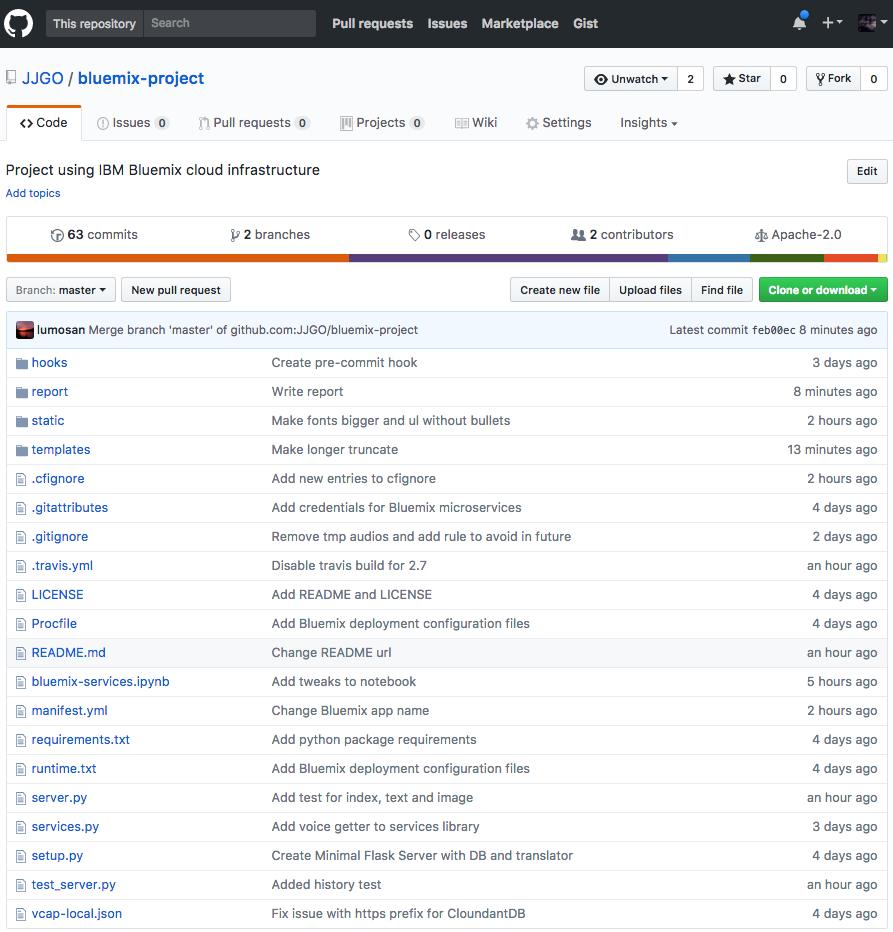
\includegraphics[width=\textwidth]{git}
\end{figure}

\begin{figure}[htp!]
    \centering
    \caption{Travis: \url{https://travis-ci.org/JJGO/bluemix-project}}
    \label{fig:travis}
    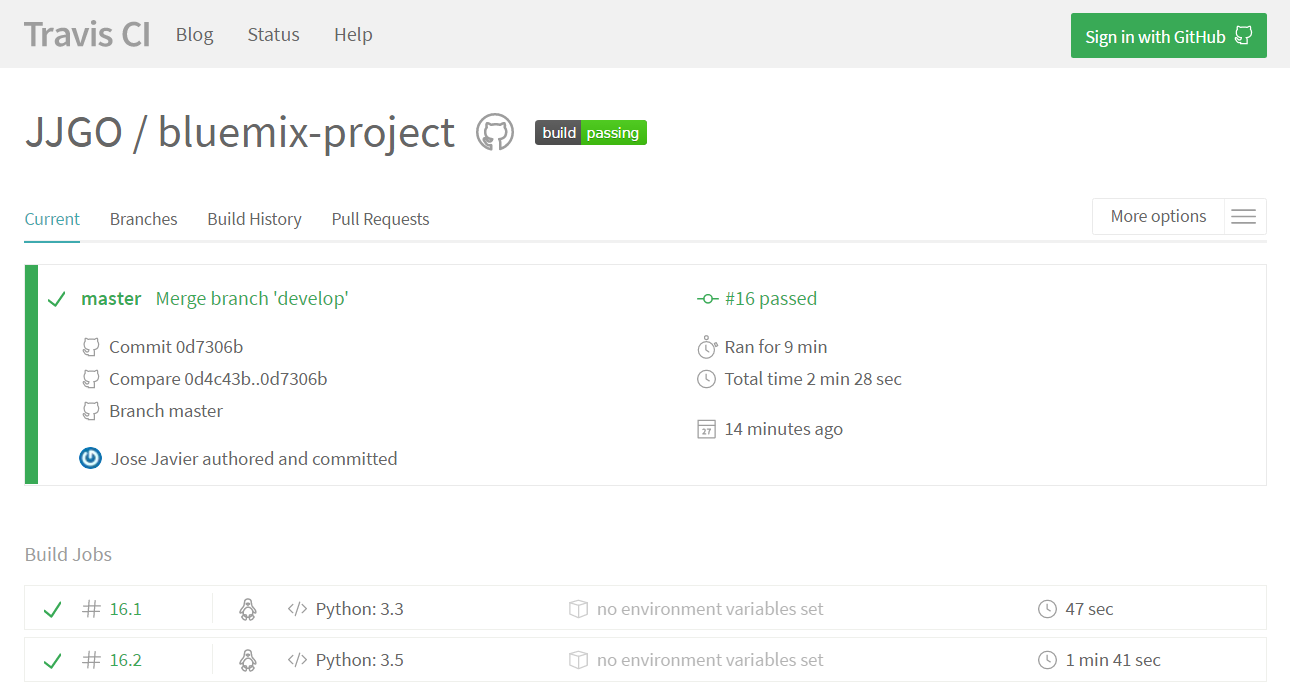
\includegraphics[width=\textwidth]{travis}
\end{figure}

\begin{figure}[htp!]
    \centering
    \caption{El uso de Integración Continua queda reflejado en GitHub, donde el código aparece como 'build:passing'}
    \label{fig:git2}
    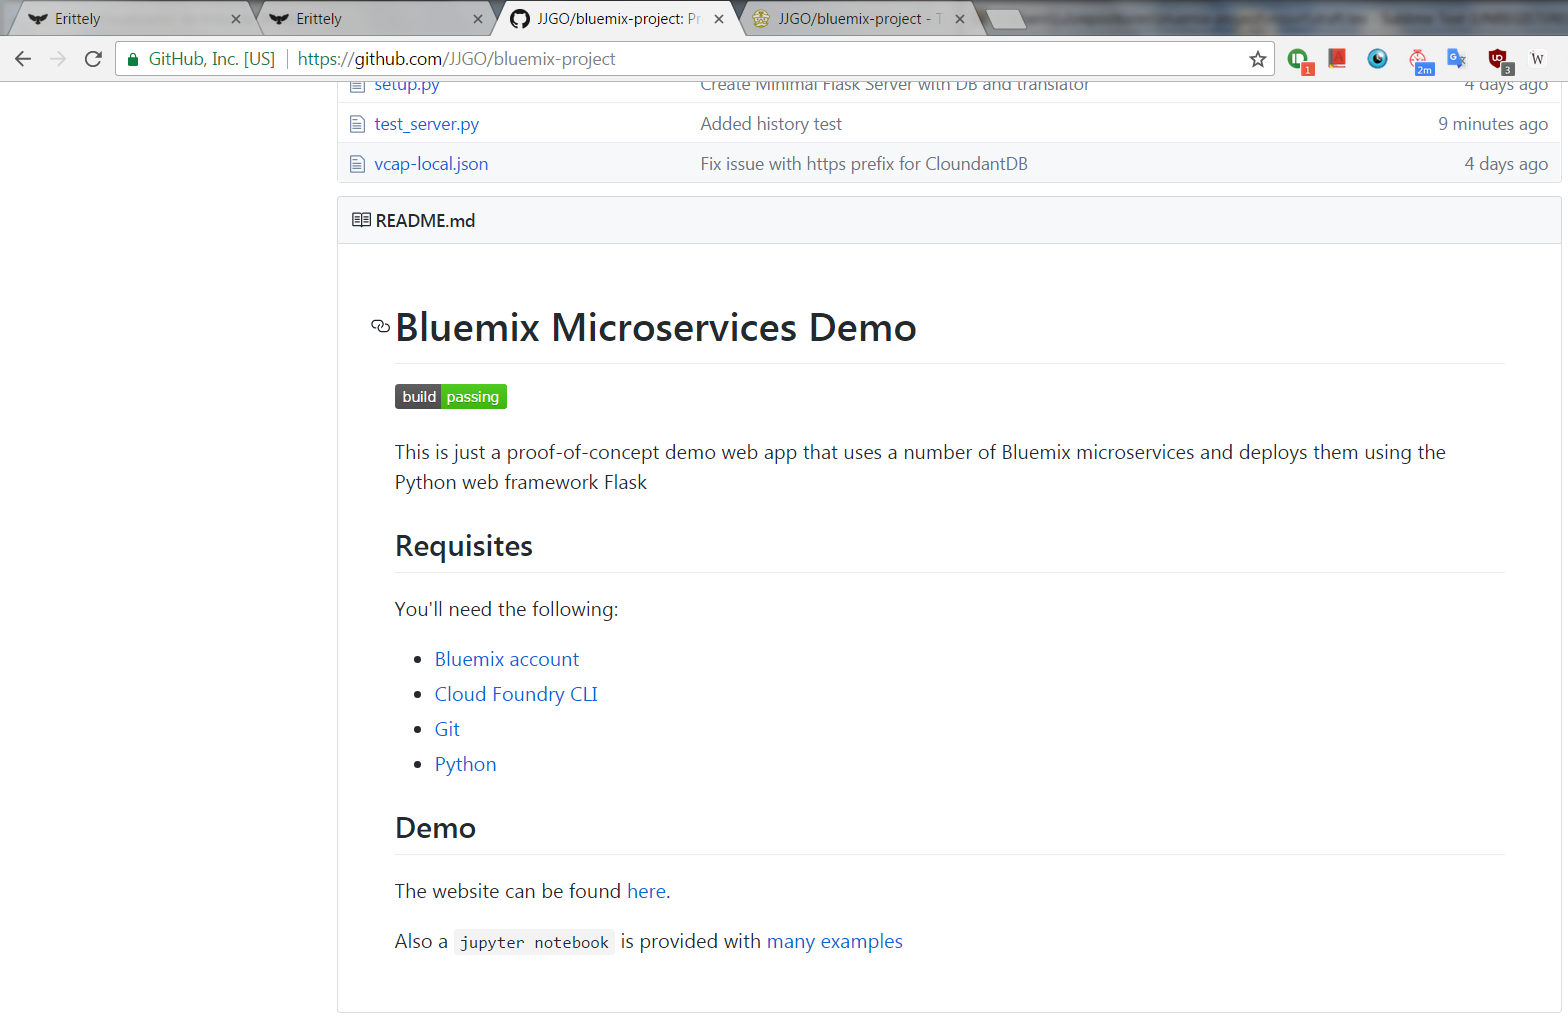
\includegraphics[width=\textwidth]{git2}
\end{figure}


% section introducción (end)
\newpage
\clearpage
\section{Capturas de pantalla de la aplicación} % (fold)
\label{sec:capturas_de_pantalla_de_la_aplicación}
\subsection{Responsividad} % (fold)
\label{sub:responsividad}

% subsection responsividad (end)
\begin{figure}[htp!]
    \centering
    \caption{Pantalla de inicio (responsividad I)}
    \label{fig:1}
    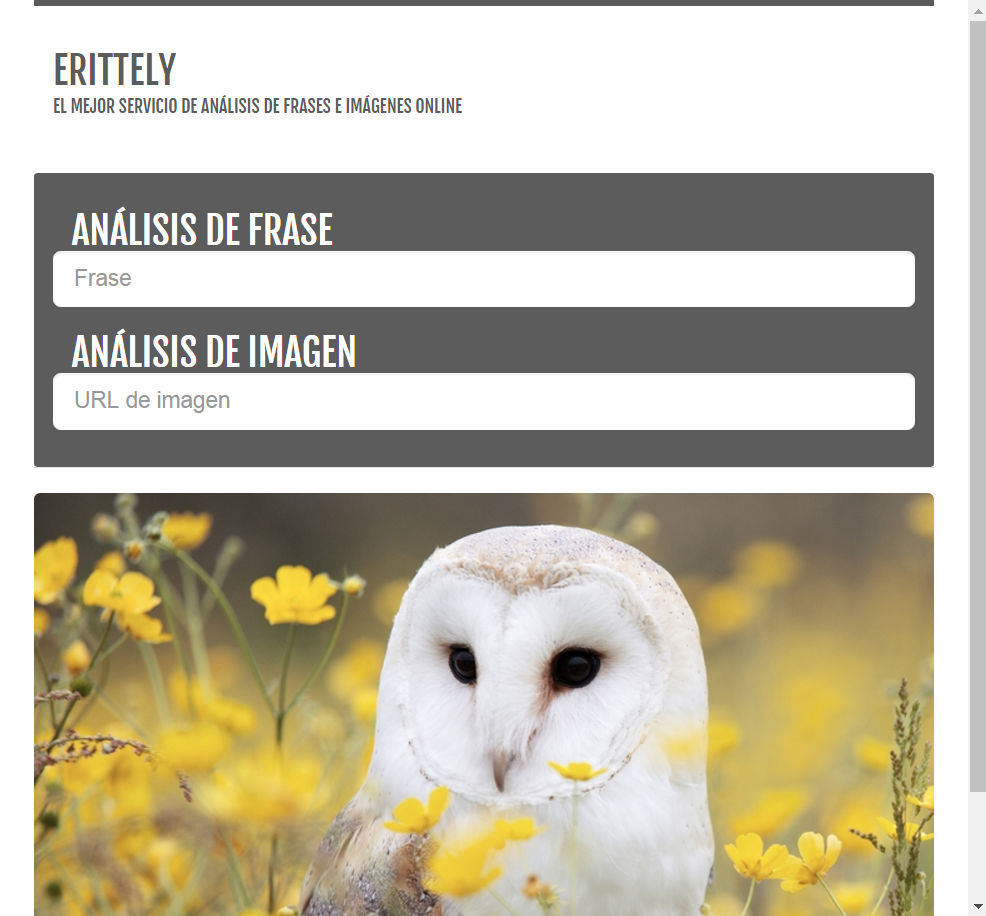
\includegraphics[width=0.7\textwidth]{1}
\end{figure}
\begin{figure}[htp!]
    \centering
    \caption{Pantalla de inicio (responsividad II)}
    \label{fig:2}
    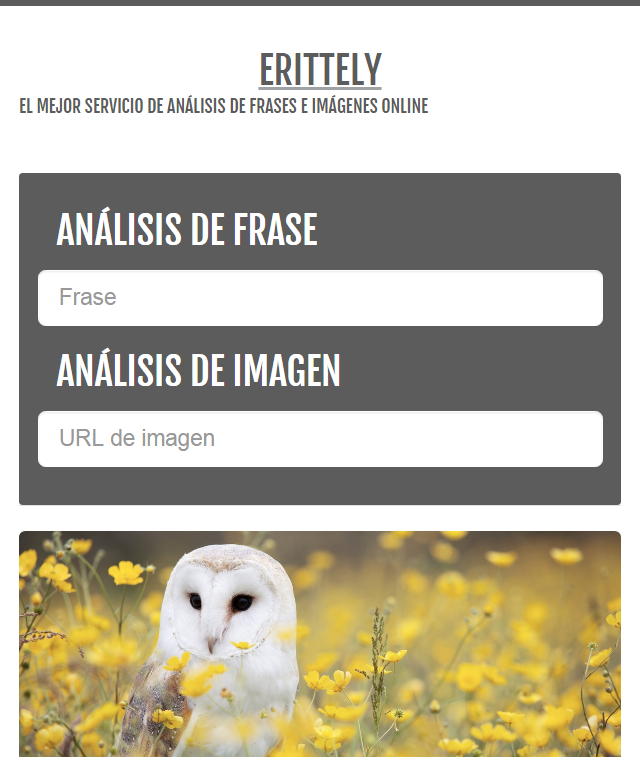
\includegraphics[width=0.5\textwidth]{2}
\end{figure}
\begin{figure}[htp!]
    \centering
    \caption{Pantalla de inicio (responsividad III)}
    \label{fig:3}
    
\includegraphics[width=0.45\textwidth]{3}
\end{figure}
\newpage
\clearpage
\subsection{Funcionamiento de la aplicación} % (fold)
\label{sub:funcionamiento_de_la_aplicación}

% subsection funcionamiento_de_la_aplicación (end)
\begin{figure}[htp!]
    \centering
    \caption{(1) Introducir frase}
    \label{fig:5}
    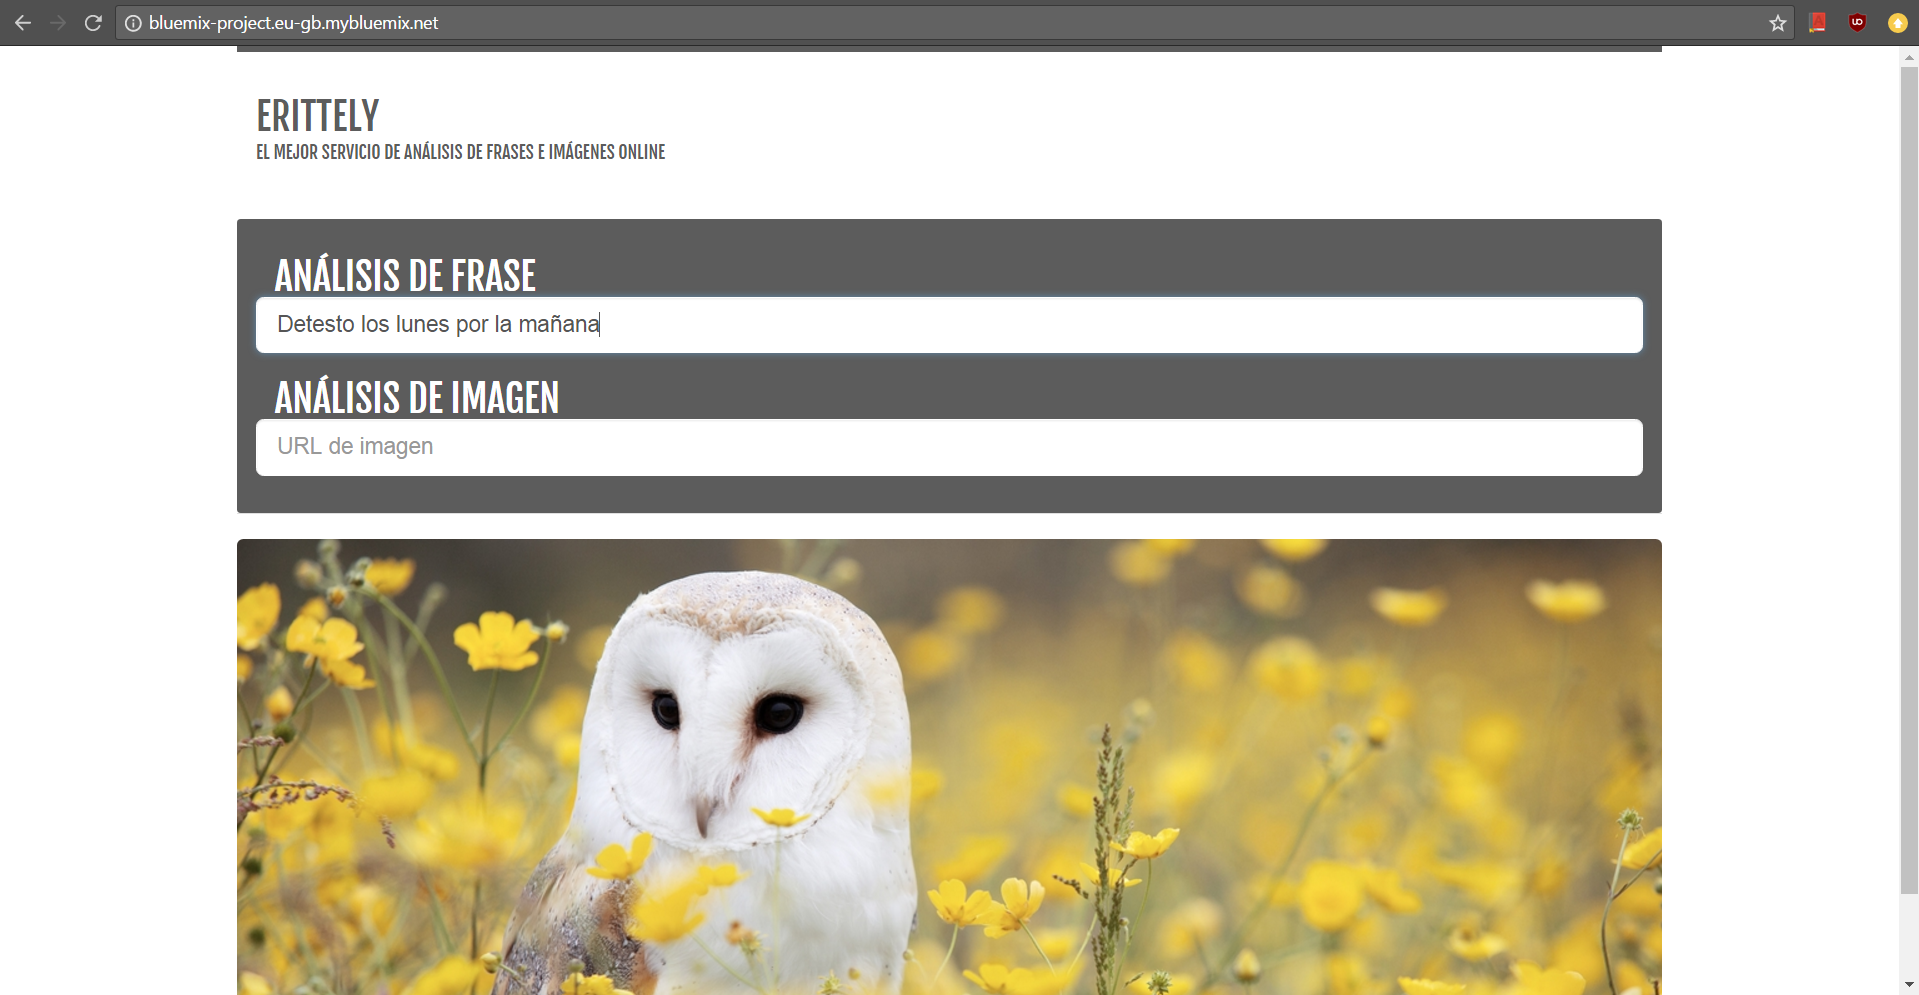
\includegraphics[width=\textwidth]{a}
\end{figure}
\begin{figure}[htp!]
    \centering
    \caption{(2) Procesamiento de la frase}
    \label{fig:6}
    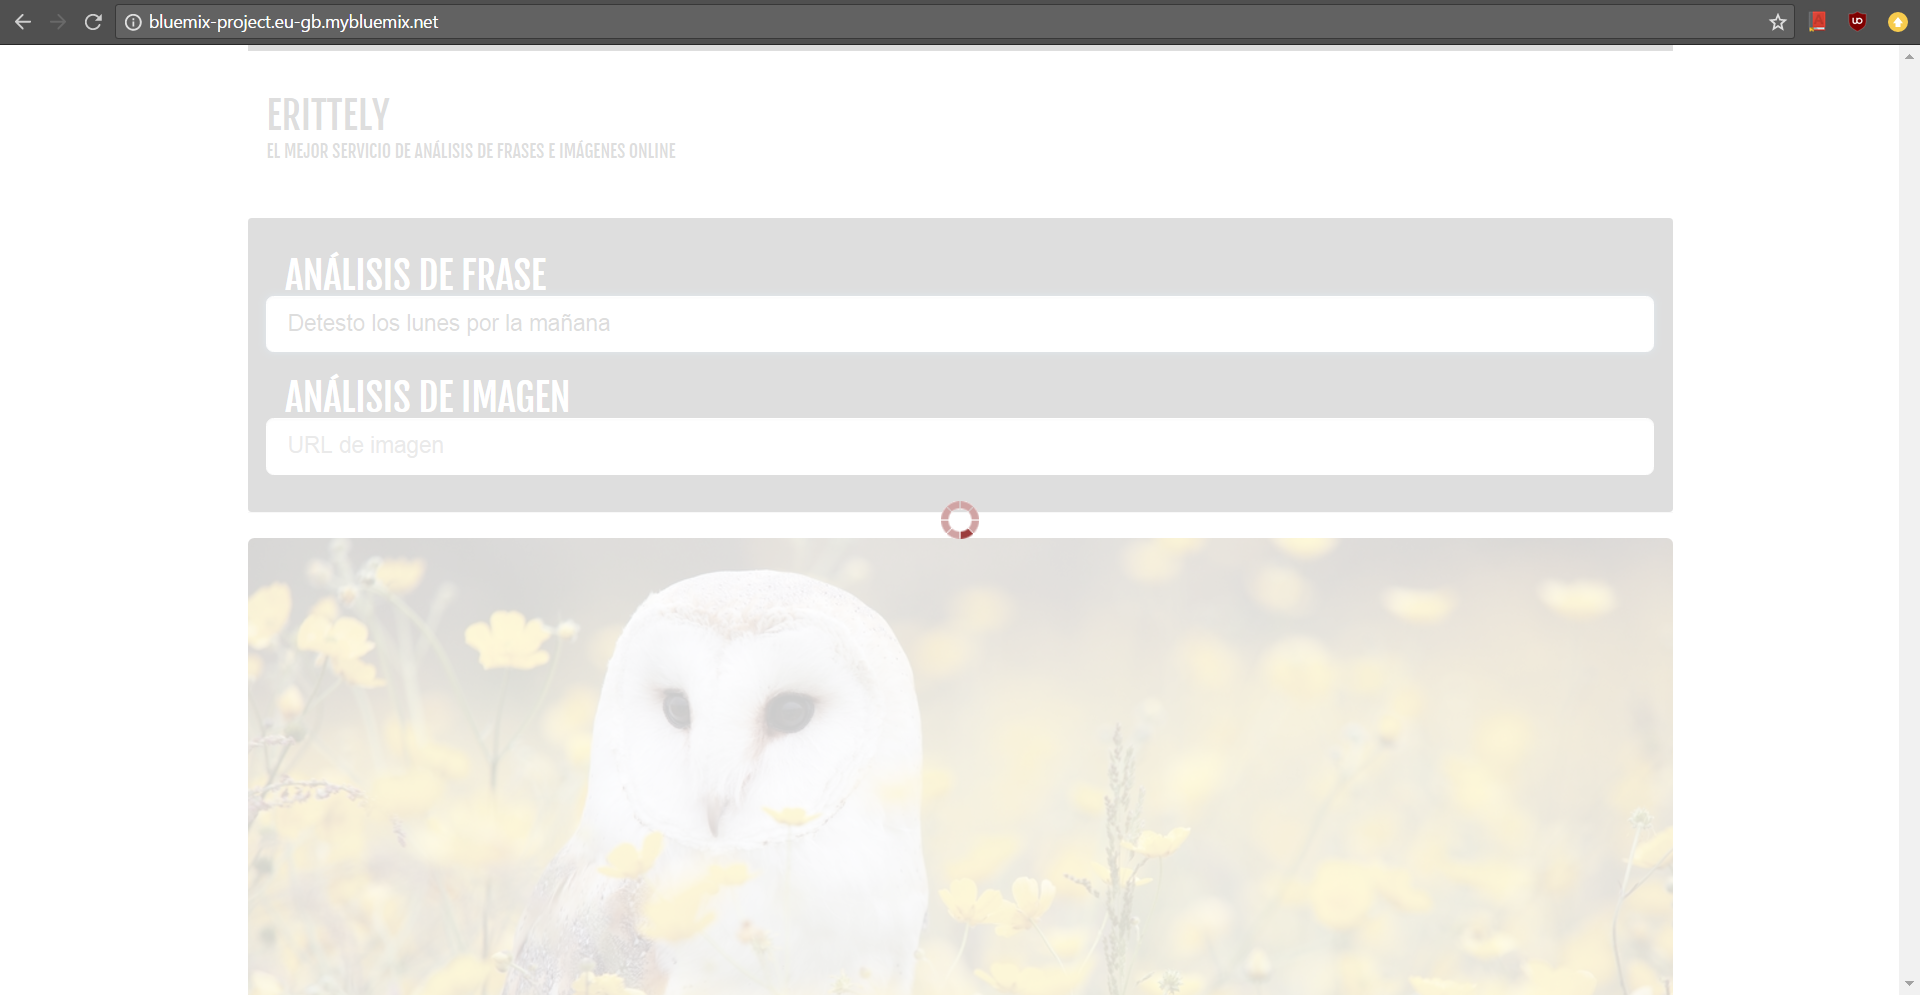
\includegraphics[width=\textwidth]{b}
\end{figure}
\begin{figure}[htp!]
    \centering
    \caption{(3) Resultado. A la derecha aparece el historial, en el que ahora se incluye esta frase.}
    \label{fig:7}
    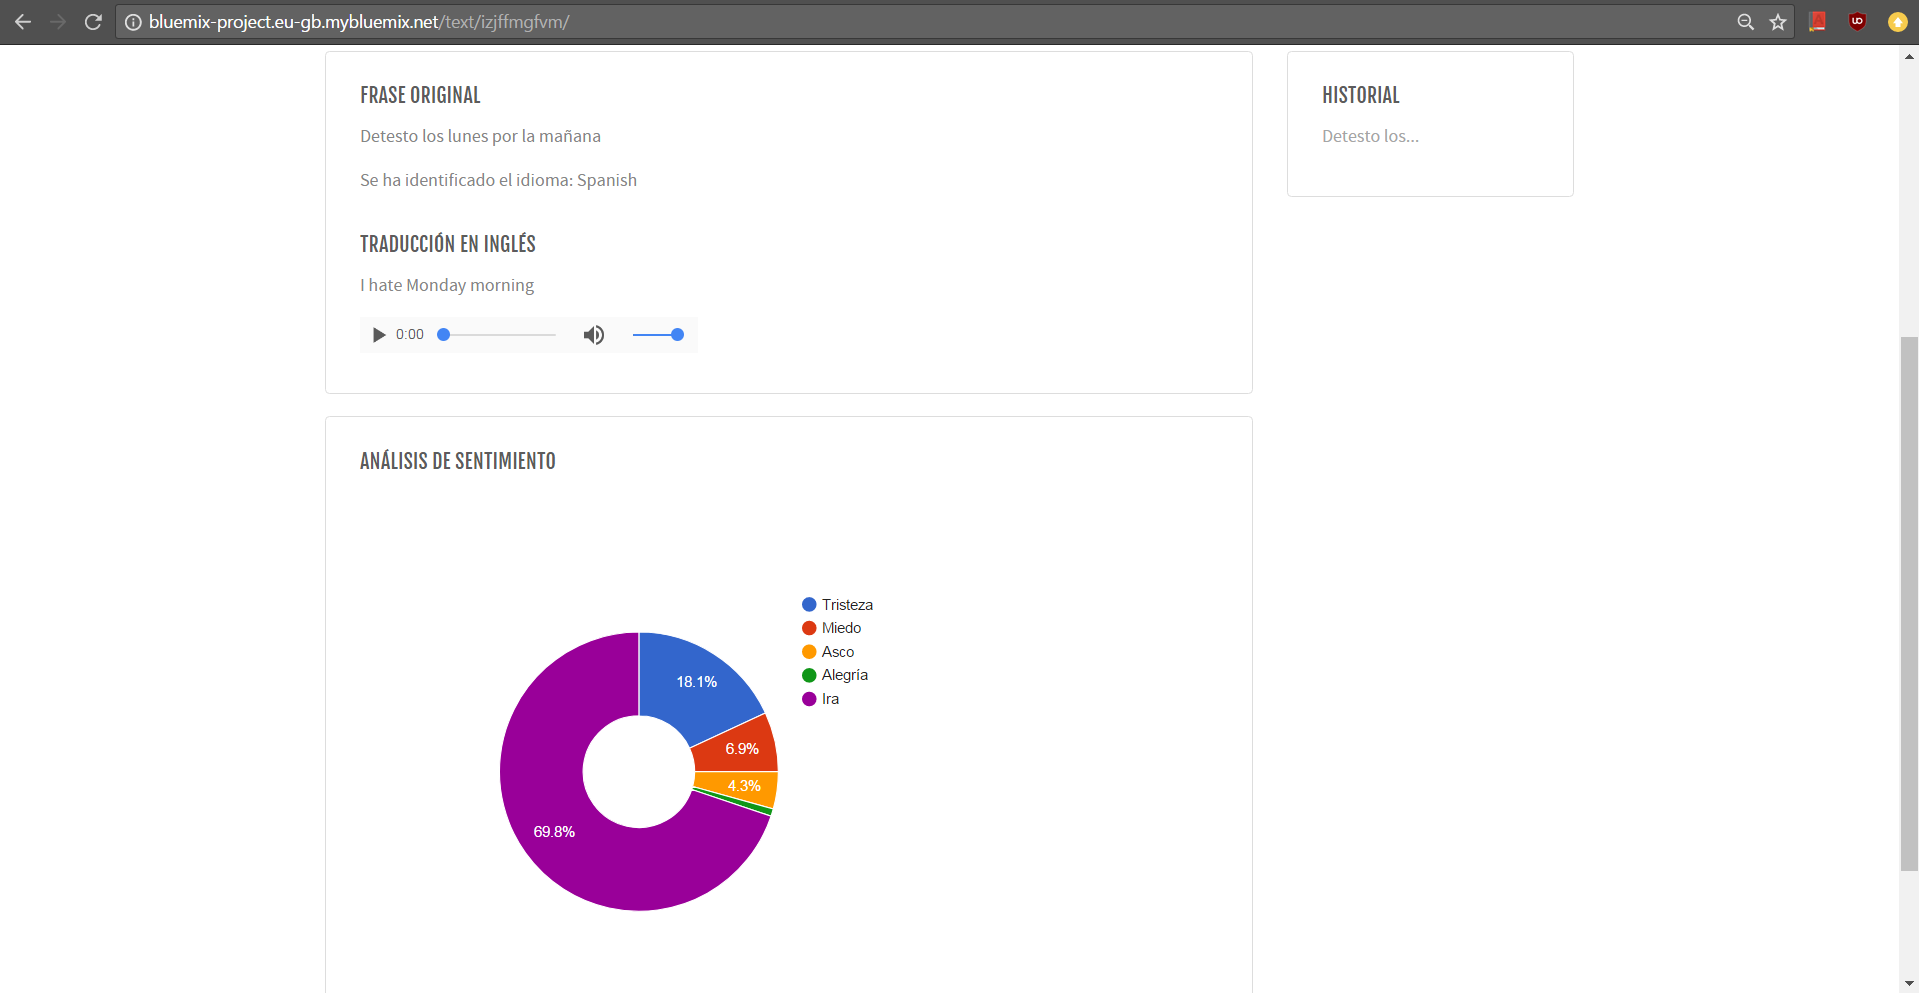
\includegraphics[width=\textwidth]{c}
\end{figure}
\begin{figure}[htp!]
    \centering
    \caption{(4) Ahora analizamos una imagen}
    \label{fig:9}
    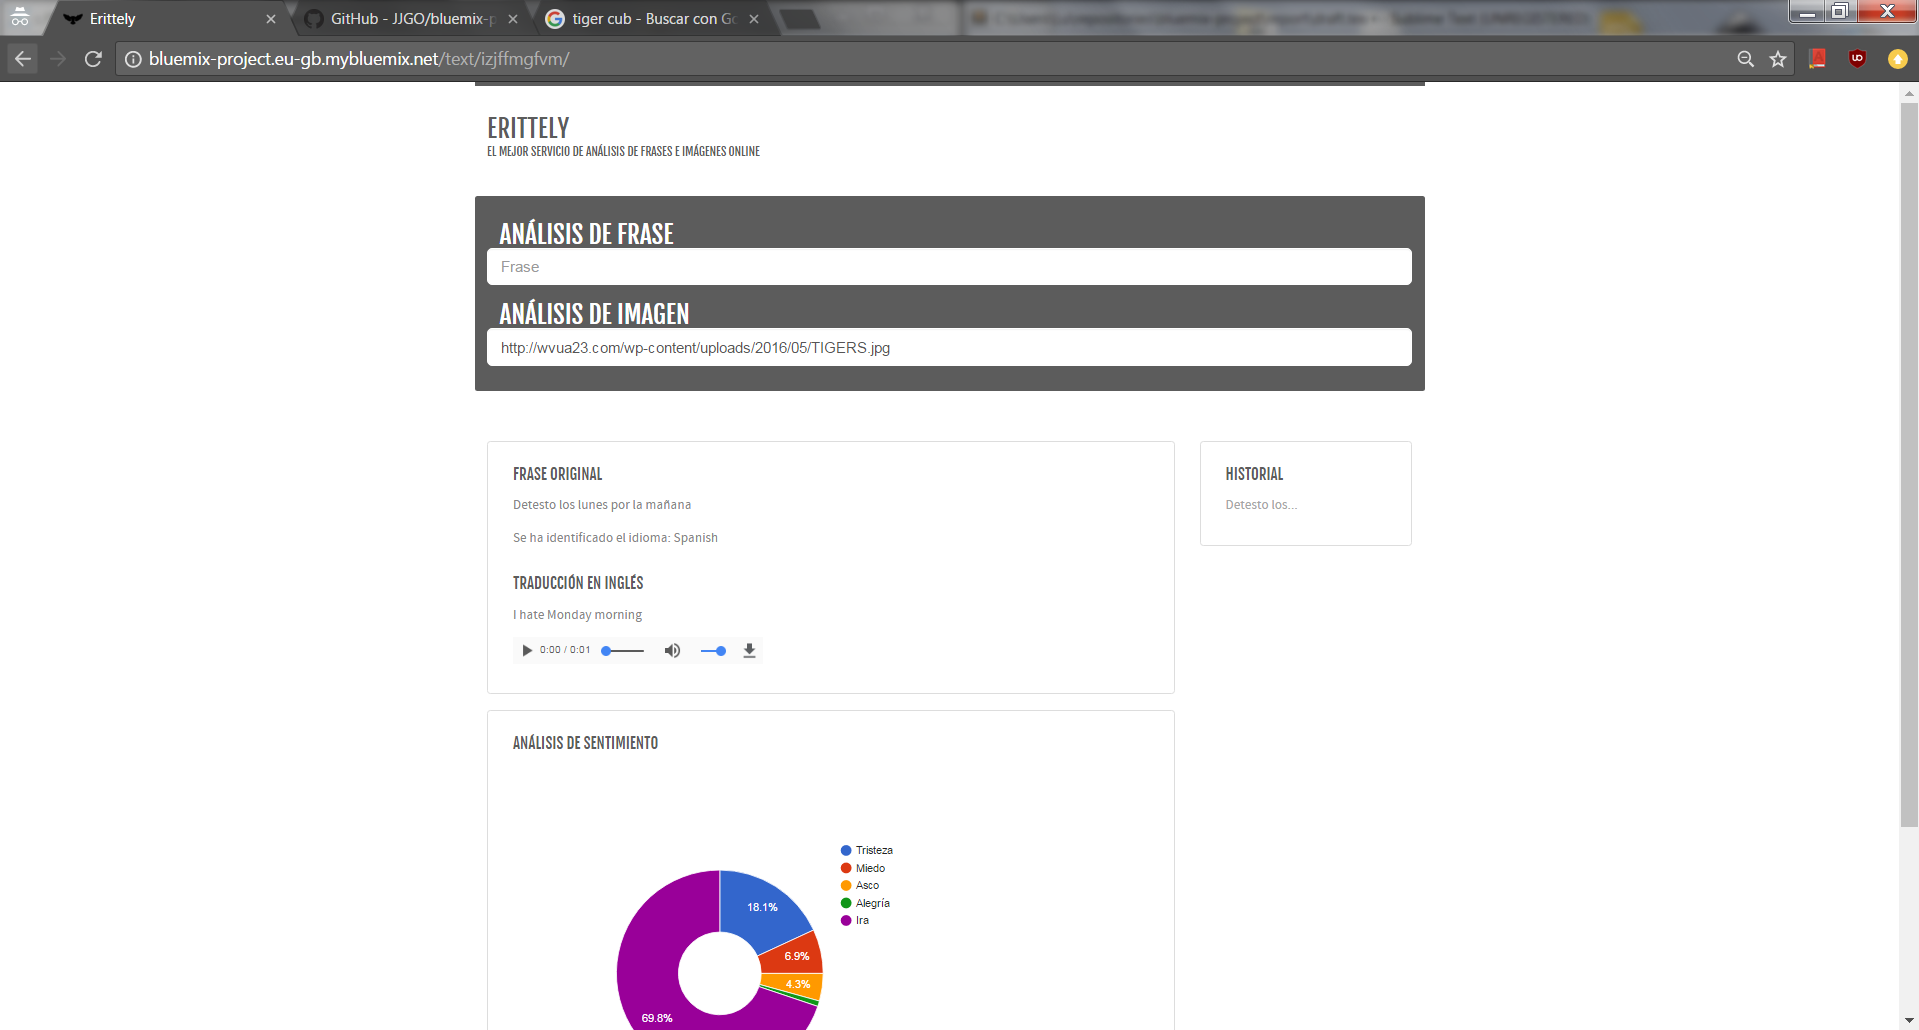
\includegraphics[width=\textwidth]{d2}
\end{figure}
\begin{figure}[htp!]
    \centering
    \caption{(5) Resultado obtenido. Se ha añadido este elemento en el historial.}
    \label{fig:10}
    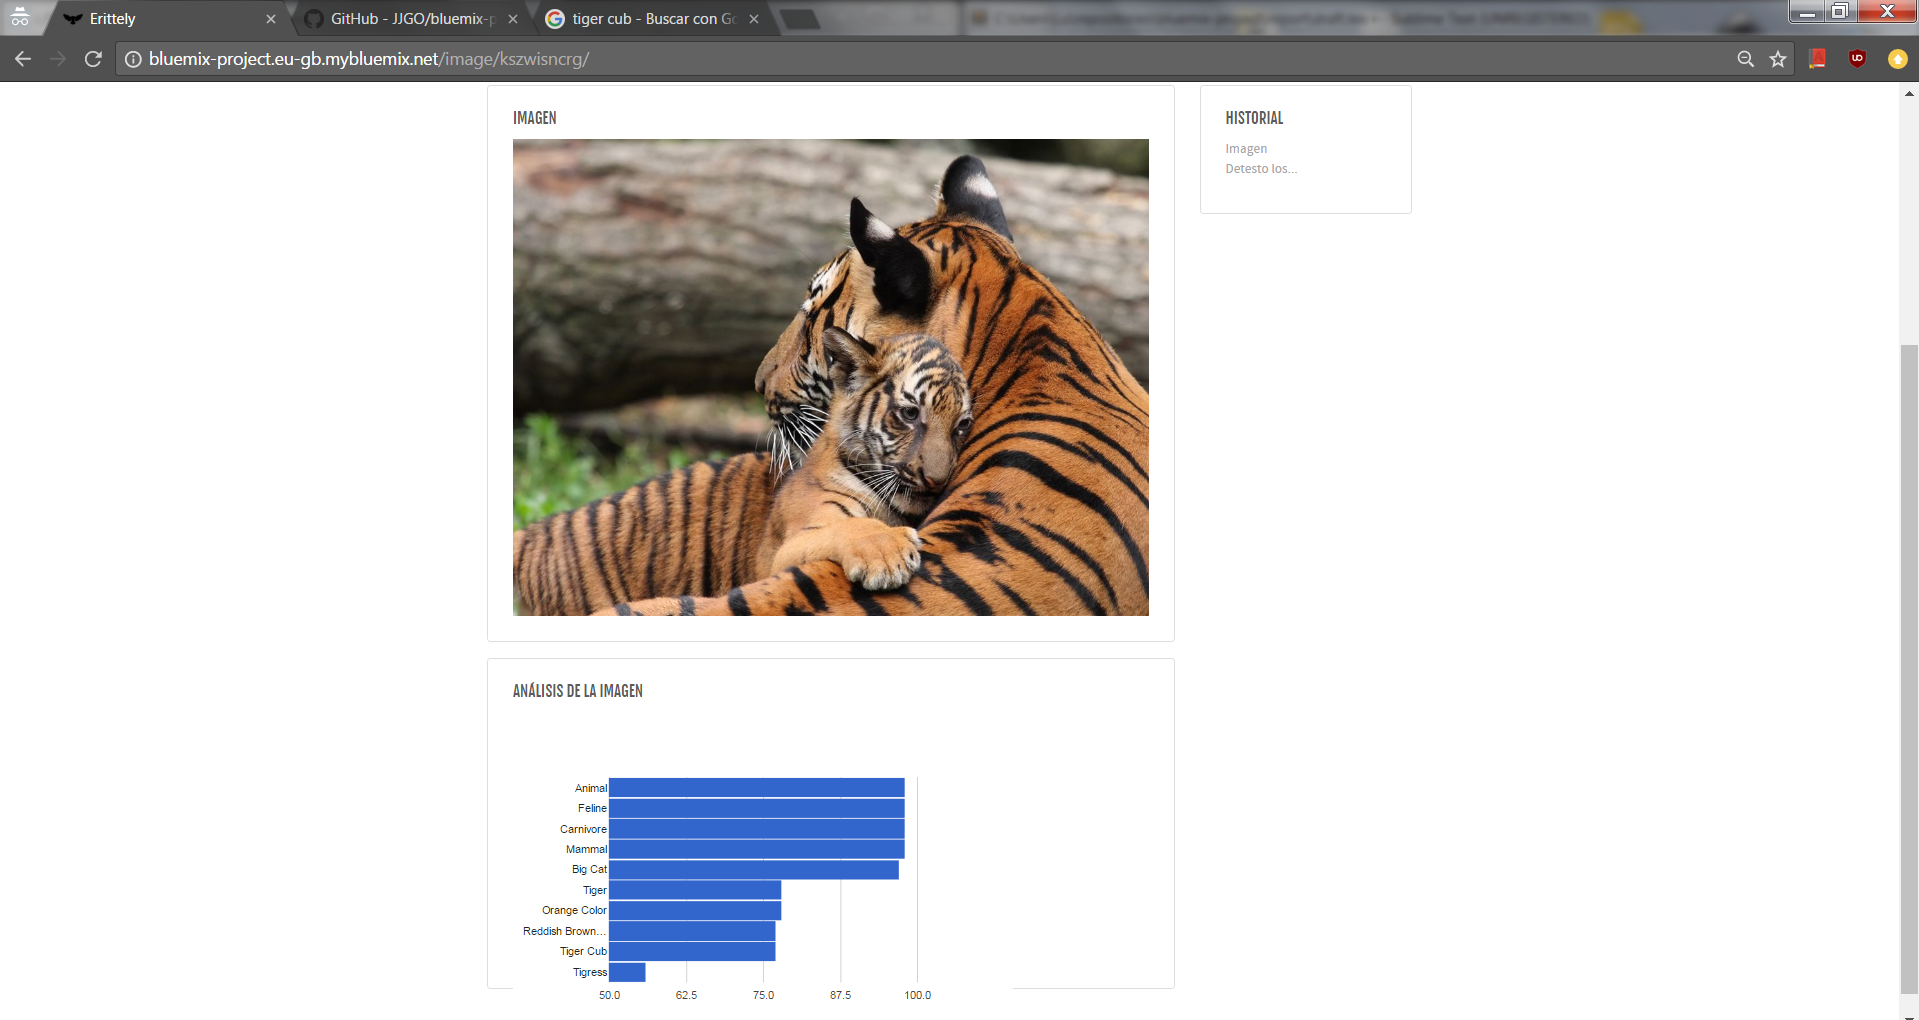
\includegraphics[width=\textwidth]{e2}
\end{figure}
\begin{figure}[htp!]
    \centering
    \caption{(6) Se puede hacer click en cualquier elemento del historial para repetir consultas anteriores}
    \label{fig:11}
    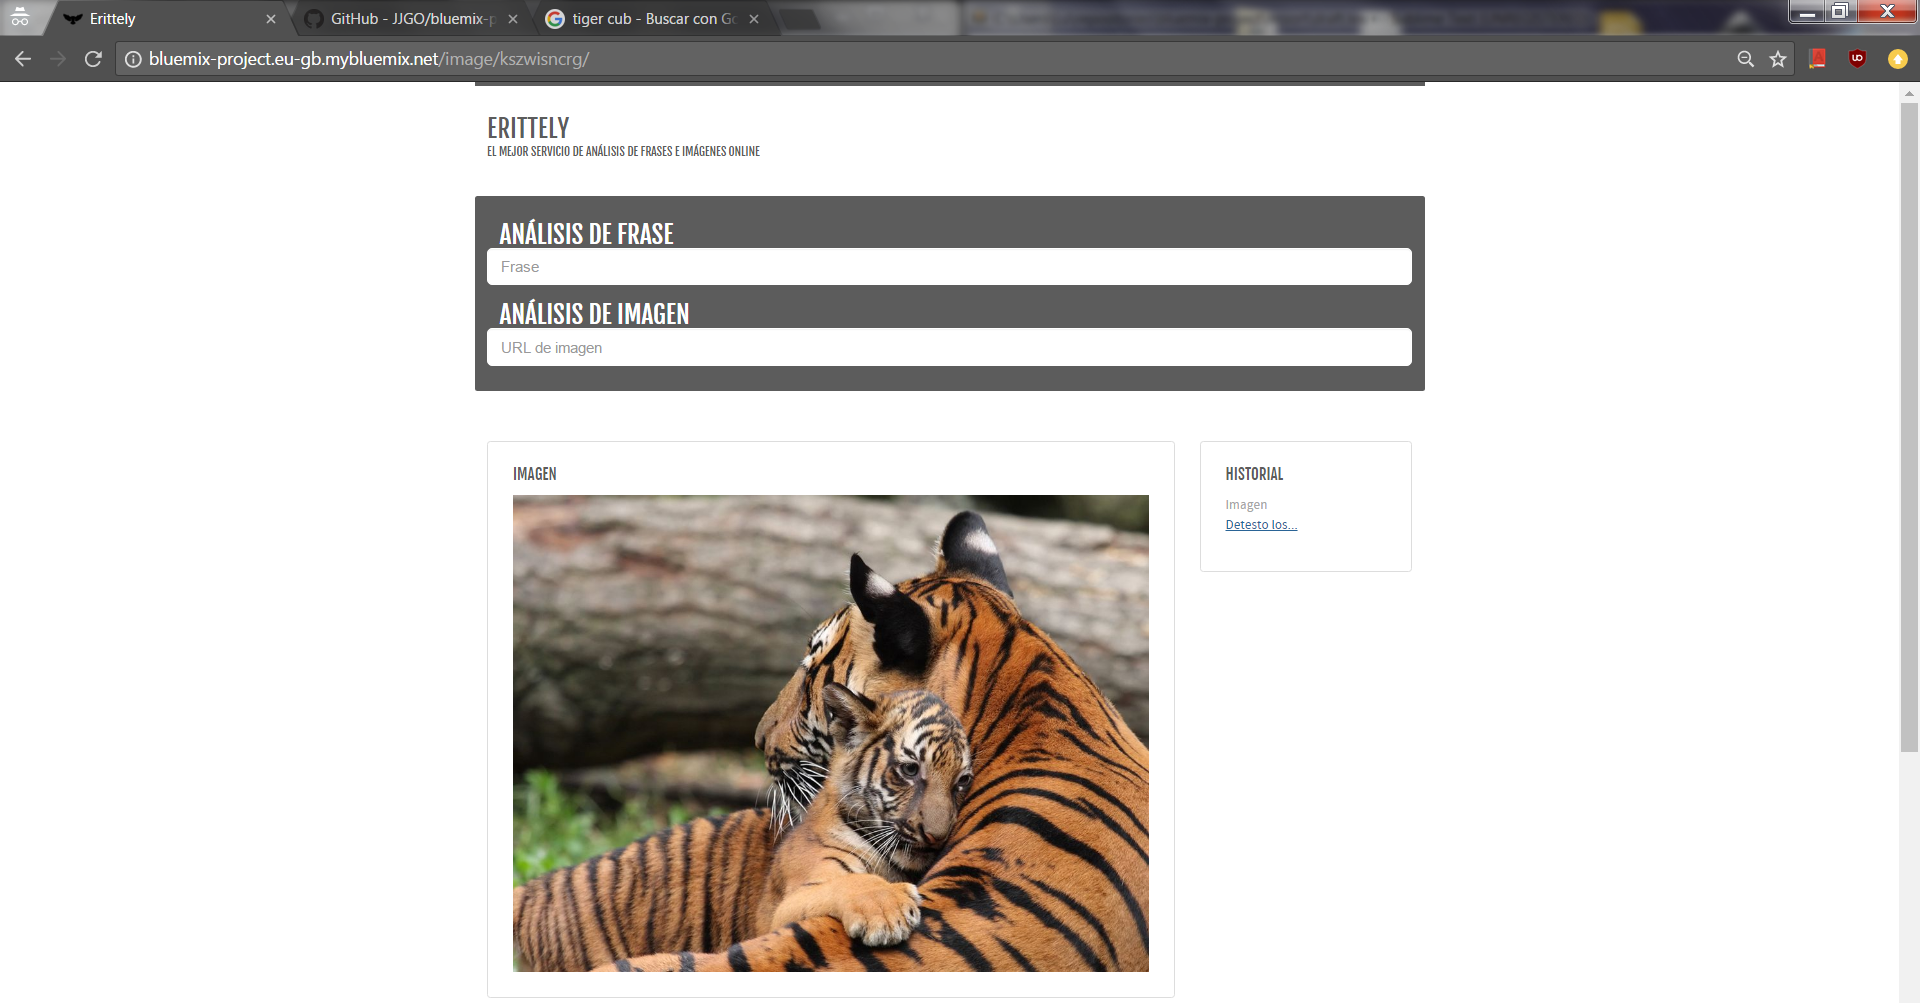
\includegraphics[width=\textwidth]{f2}
\end{figure}

\begin{figure}[htp!]
    \centering
    \caption{(7) Se repite la consulta anterior, y el elemento correspondiente del historial se coloca como el más reciente}
    \label{fig:11}
    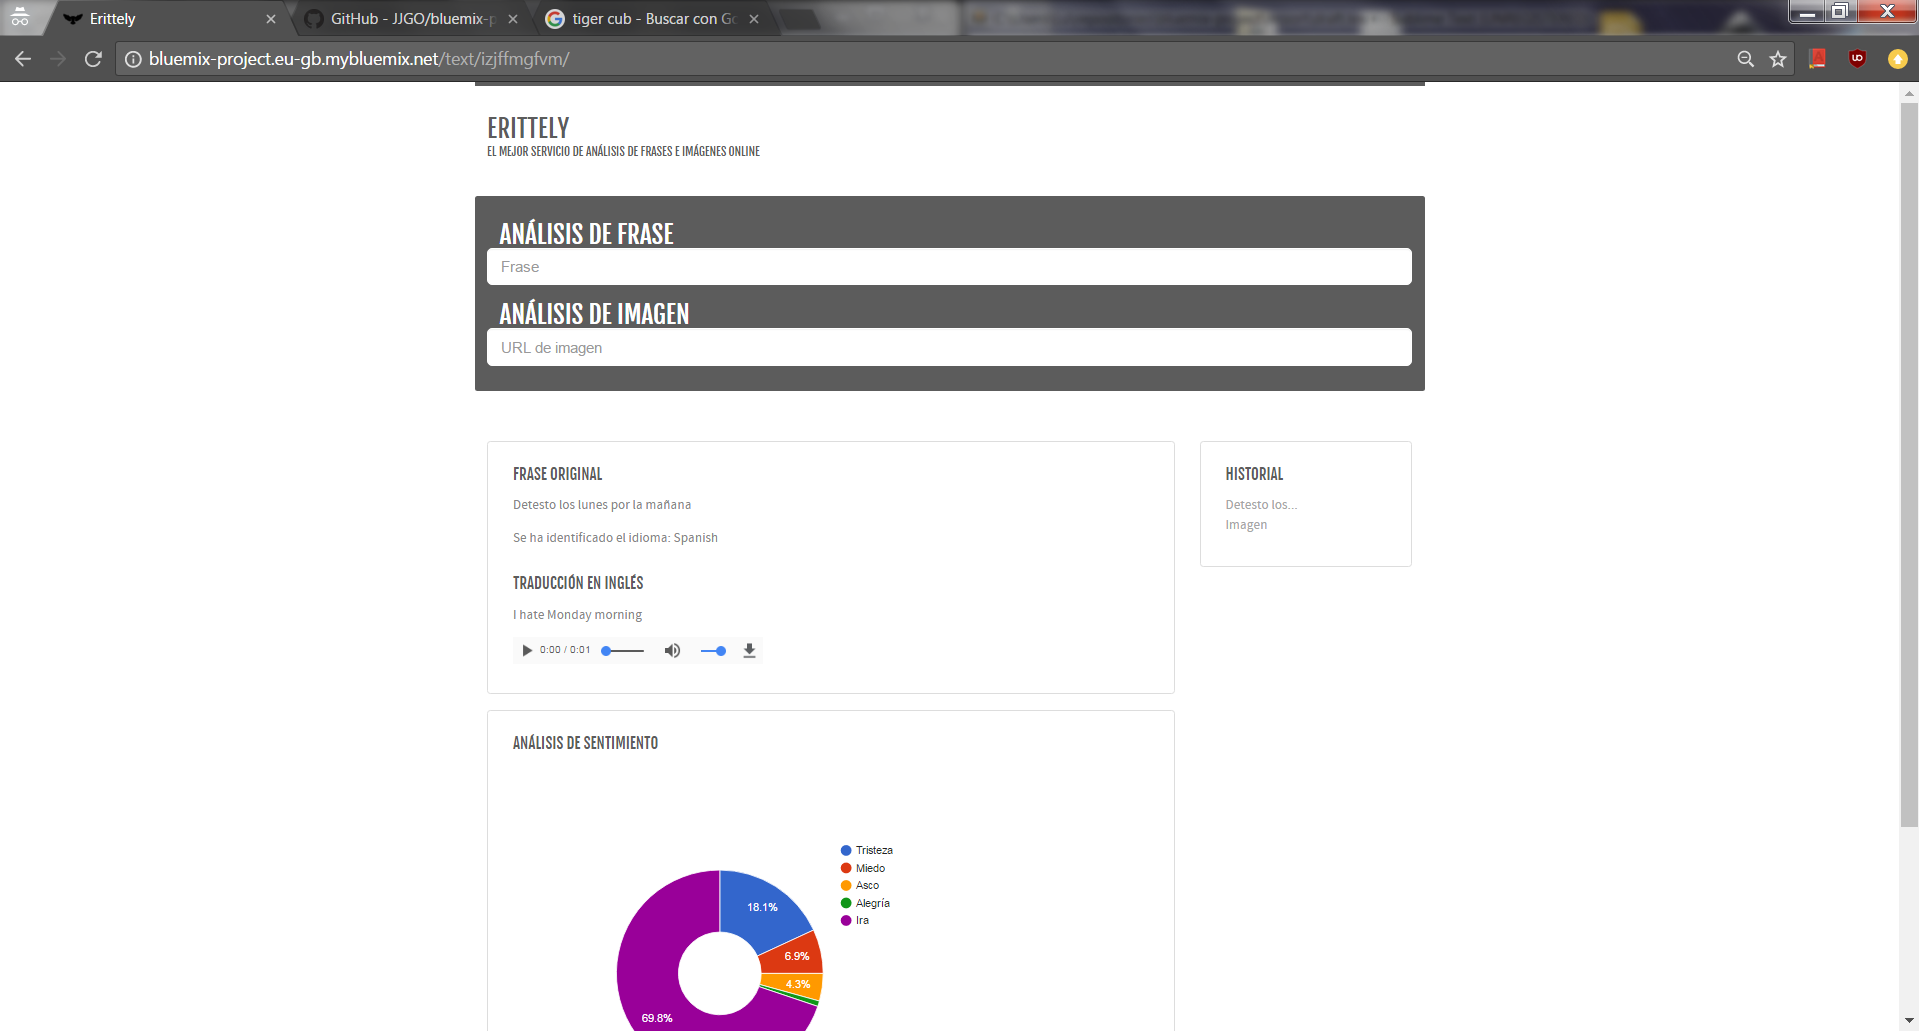
\includegraphics[width=\textwidth]{g}
\end{figure}
% section capturas_de_pantalla_de_la_aplicación (end)
\end{document}
